\section{Diskussion und Ausblick} \label{chap:Diskussion und Ausblick}
In diesem Kapitel werden die Auswirkungen der Ergebnisse der Bachelorarbeit, wichtige Aspekte, mögliche fortführende Forschungen und weitere Verteidigungsmechanismen diskutiert. 

\subsection{Auswirkungen unserer Ergebnisse}

Die Ergebnisse dieser Studie unterstreichen die anhaltende Herausforderung bei der \Gls{robustifizierung} von Modellen gegen \acrlong{uap}s (\acrshort{uap}s) und Adversarial Attacks im Allgemeinen. Der entwickelte Robustifizierungsmechanismus kann bedingt ein Modell gegen Angriffe schützen, dies verdeutlicht  die Notwendigkeit, weiterhin intensive Forschung in diesem Bereich zu betreiben.

Die zunehmende Grösse und Komplexität moderner Modelle führt zu einer steigenden Undurchsichtigkeit der Entscheidungsprozesse. Dies erschwert nicht nur das Verständnis der Modellentscheidungen, sondern auch die Erkennung potenzieller Schwachstellen gegenüber Adversarial Attacks. In diesem Kontext könnte die Integration von Explainable AI-Techniken und/oder Bildsegmentierungssystemen einen vielversprechenden Ansatz darstellen.

Durch die Nutzung von Explainable AI könnten die Entscheidungsprozesse der Modelle transparenter gestaltet werden. Dies würde es ermöglichen, die Logik hinter den Modellentscheidungen besser nachzuvollziehen und somit auch unplausible oder inkonsistente Ausgaben, die auf Adversarial Attacks hindeuten könnten, leichter zu identifizieren. Bildsegmentierungssysteme könnten zusätzlich dazu beitragen, subtile Veränderungen in den Eingabedaten zu erkennen, die auf \acrshort{uap}s oder andere Arten von Adversarial Attacks hinweisen.

Die Kombination dieser Ansätze mit menschlicher Expertise könnte eine effektivere Strategie zur Erkennung und Abwehr von dieser Angriffe darstellen. Insbesondere in kritischen Anwendungsbereichen, wo die Konsequenzen falscher Entscheidungen schwerwiegend sein können, ist es essenziell, dass Menschen in der Lage sind, die Plausibilität der Modellentscheidungen zu überprüfen und potenzielle Anomalien zu erkennen.

Zukünftige Forschungsarbeiten sollten sich daher nicht nur auf die Verbesserung der direkten Robustifizierungsmethoden konzentrieren, sondern auch auf die Entwicklung integrierter Ansätze, die Explainable AI, fortschrittliche Bildanalysetechniken und menschliche Überwachung kombinieren. Dies könnte zu resilienteren KI-Systemen führen, die sowohl robuster gegen Adversarial Attacks als auch transparenter und nachvollziehbarer in ihren Entscheidungsprozessen sind.

\subsection{Black-Box-Attacken}
Wie im Kapitel \ref{chap:Universal Adversarial Attacks auf Bildklassifikation} beschrieben, ist der in dieser Arbeit beschriebener Perturbationsalgorithmus eine White-Box-Attacke. Im Paper von Moosavi-Dezfooli et al.
\cite{moosavi-dezfooli_universal_2017} wird jedoch auch die Generalisierbarkeit thematisiert. Sie stellten fest, dass \acrshort{uap}s, die für ein bestimmtes Modell A (z.B. VGG-19) generiert wurden, auch bei einem anderen Modell B (z.B. ResNet-152) zu Fehlklassifikationen führen können.

Diese Beobachtung eröffnet die Möglichkeit, effektive Perturbationen zu erzeugen, ohne Kenntnis der genauen Modellgewichte oder der spezifischen Architektur zu haben. Somit können auch Black-Box-Attacken durchgeführt werden, bei denen der Angreifer keinen direkten Zugriff auf das interne Modell hat. 

\subsection{Mögliche fortführende Forschungen}
Als weiterführende Forschung könnten die Methoden zur Bias-Detektion (\ref{chap:bias-detektion}) und Multiklassifikation (\ref{chap:multiklassifikation}) auf einen anderen Datensatz angewendet werden.

\subsubsection{Bias Detektion} \label{chap:bias-detektion}
Bei der Generierung von \acrlong{uap}s für das Modell ResNet50 und den Datensatz COVIDx CXR-4 in der Abbildung \ref{fig:bias-detektion} ist zu erkennen, dass sich die generierten Perturbationen hauptsächlich in der oberen rechten Ecke konzentrieren.

\begin{figure}[H]
    \centering
    \begin{subfigure}{0.19\linewidth}
        \centering
        
\includegraphics[height=1\linewidth]{01-images/05-resultate/uap_resnet50/uap0-resnet50-covidx_data-n200-robustificationslevel0.png}
    \end{subfigure}\hfill%
    \begin{subfigure}{0.19\linewidth}
        \centering
        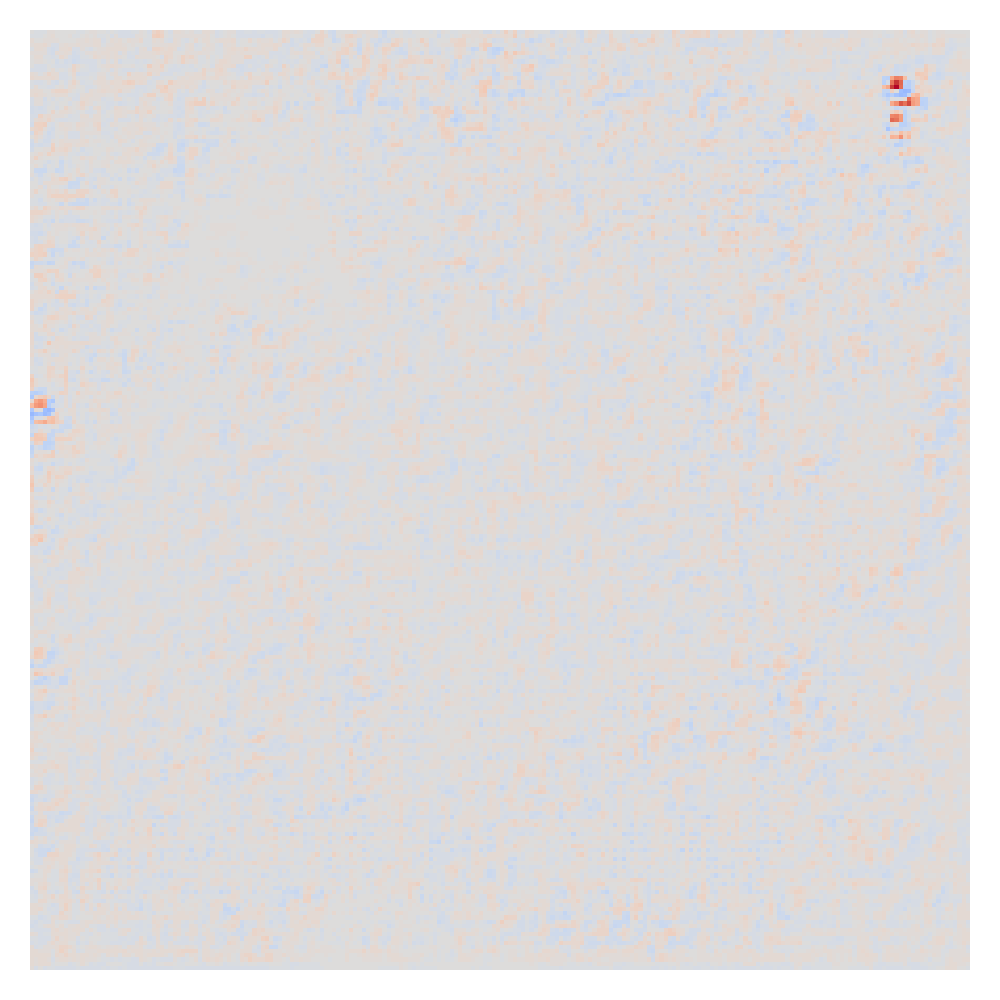
\includegraphics[height=1\linewidth]{01-images/05-resultate/uap_resnet50/uap1-resnet50-covidx_data-n200-robustificationslevel0.png}
    \end{subfigure}\hfill%
    \begin{subfigure}{0.19\linewidth}
        \centering
        
\includegraphics[height=1\linewidth]{01-images/05-resultate/uap_resnet50/uap2-resnet50-covidx_data-n200-robustificationslevel0.png}
    \end{subfigure}\hfill%
    \begin{subfigure}{0.19\linewidth}
        \centering
        
\includegraphics[height=1\linewidth]{01-images/05-resultate/uap_resnet50/uap3-resnet50-covidx_data-n200-robustificationslevel0.png}
    \end{subfigure}\hfill%
    \begin{subfigure}{0.19\linewidth}
        \centering
        
\includegraphics[height=1\linewidth]{01-images/05-resultate/uap_resnet50/uap4-resnet50-covidx_data-n200-robustificationslevel0.png}
    \end{subfigure}\hfill%
    \caption{\acrlong{uap}s des Modells ResNet50 auf den Datensatz COVIDx CXR-4}
    \label{fig:bias-detektion}
\end{figure}

Da der Perturbationsalgorithmus hauptsächlich an dieser Stelle angreift, könnte daraus geschlossen werden, dass dieser Bildbereich für die Klassifikation sehr wichtig ist. Sollte dies tatsächlich der Fall sein, könnte die Erzeugung solcher \acrshort{uap}s alternativ zu Grad-CAM zur Aufdeckung von Bias oder zur Erklärbarkeit von Bildklassifikationsmodellen verwendet werden. 

Die hier getroffenen Annahmen müssten jedoch überprüft werden.

\subsubsection{Multiklassifkation} \label{chap:multiklassifikation}
In dieser Arbeit werden binäre Klassifikationsmodelle analysiert. Während binäre Klassifikationsmodelle ein einziges Neuron mit einer Sigmoid-Aktivierungsfunktion im letzten Layer besitzen, zeichnen sich Multiklassifikationsmodelle durch die Integration mehrerer Neuronen aus, die mittels einer Softmax-Funktion aktiviert werden. Die genannten Unterschiede in der Architektur machen die Anwendung angepasster Methoden zum Täuschen solcher Modelle erforderlich.

Während bei binären Klassifikationen die Binary Cross Entropy als Loss-Funktion dient, wird bei Multiklassifikationsmodellen die Cross Entropy Funktion verwendet werden. Die Cross Entropy Funktion eignet sich für die Bewertung von Wahrscheinlichkeitsverteilungen über alle Klassenkategorien hinweg.

\begin{equation}
    L_{\text{UAP,MC,U}} = \frac{1}{L_{\text{CE,UAP}}(y_i, \hat{y}_{i,\text{adv}}) + \epsilon} + \lambda_{norm} \cdot ||v + \Delta v||_p 
\label{eq:Loss L_UAP_CE}
\end{equation}

\begin{equation}
L_{\text{CE,UAP}} = -\sum_{c=1}^My_{i,c}\log(\hat{y}_{i,\text{adv},c})
\label{eq:Loss L_CE_UAP}
\end{equation}

\begin{align*}
M,                &\text{ Gesamtanzahl Klassen.} \\
c,                &\text{ Klassenlabel.} \\
y_{i,c},          &\text{ Label des i-ten Datenpunkts für Klasse c.} \\
\hat{y}_{i,\text{adv},c},    &\text{ Vorhersage des Modells $f(x_{i,\text{adv}})$ des i-ten Datenpunkts für Klasse c.} \\
\end{align*}

Diese Loss-Funktion führt einen untargeted Attack durch, indem sie eine Perturbation sucht, die die Klassifikation der ursprünglichen Klasse minimiert. Die Loss-Funktion kann jedoch auch so angepasst werden, dass sie zu einem targeted Attack führt. Dabei wird eine Perturbation gesucht, die das Modell dazu bringt, eine andere, spezifische Klasse vorherzusagen.

\begin{equation}
    L_{\text{UAP,MC,T}} = L_{\text{CE,UAP,T}}(y_{i,\text{wrong}}, \hat{y}_{i,\text{adv}}) + \lambda_{norm} \cdot ||v + \Delta v||_p 
\label{eq:Loss L_UAP_CE_Targeted}
\end{equation}

\begin{equation}
L_{\text{CE,UAP,T}} = -\sum_{c=1}^M y_{i,\text{wrong},c}\log(\hat{y}_{i,\text{adv},c})
\label{eq:Loss L_CE}
\end{equation}

Wobei $y_{i,\text{wrong}}$ für ein One-Hot-Encoded Label steht, welches einen falschen Klassenwert darstellt ($y_\text{wrong} \neq y$).

\subsection{Weitere Verteidigungsmechanismen} \label{chap:Weitere Verteidigungsmechanismen}
In dieser Arbeit wird das im Kapitel \ref{chap:adversarial training} beschriebene Adversarial Training verwendet, um das Klassifikationsmodell robuster gegen Adversarial Attacks zu machen. In den letzten Jahren wurde an weiteren Methoden geforscht, um Modelle gegen Adversarial Attacks zu schützen, welche auch gegen \acrlong{uap} getestet werden können.

\subsubsection{Cropshift Adversarial Training} \label{chap:Data Augementation}
Lin Li und Michael W. Spratling \cite{li_data_2022} präsentieren 2023 eine Data Augmentation Adversarial Training Methode namens Cropshift, die im Gegensatz zu allen bisherigen Data Augmentation Adversarial Training Methoden sowohl die Robustheit als auch die Genauigkeit des Modells verbessert. Cropshift schneidet zufällig Teile eines Bildes aus und verschiebt sie an verschiedene Positionen. Dies hilft, robustes Overfitting im Adversarial Training zu reduzieren.

\subsubsection{Ensembles mit Diversity Training} 
Sanjay Kariyappa und Moinuddin K. Qureshi \cite{kariyappa_improving_2019} zeigen, dass die Robustheit von Deep Neural Networks gegenüber Adversarial Attacks verbessert werden kann, indem ein Ensemble von Modellen mit unkorrelierten Verlustgradienten trainiert wird. Dies wird durch Diversity Training erreicht, das die gemeinsame adversarielle Subspace der Modelle reduziert und somit die Transferierbarkeit adversarieller Beispiele verringert und somit das Ensemble gegenüber Adversarial Attacks robuster ist. 

\begin{figure}[H]
    \centering
    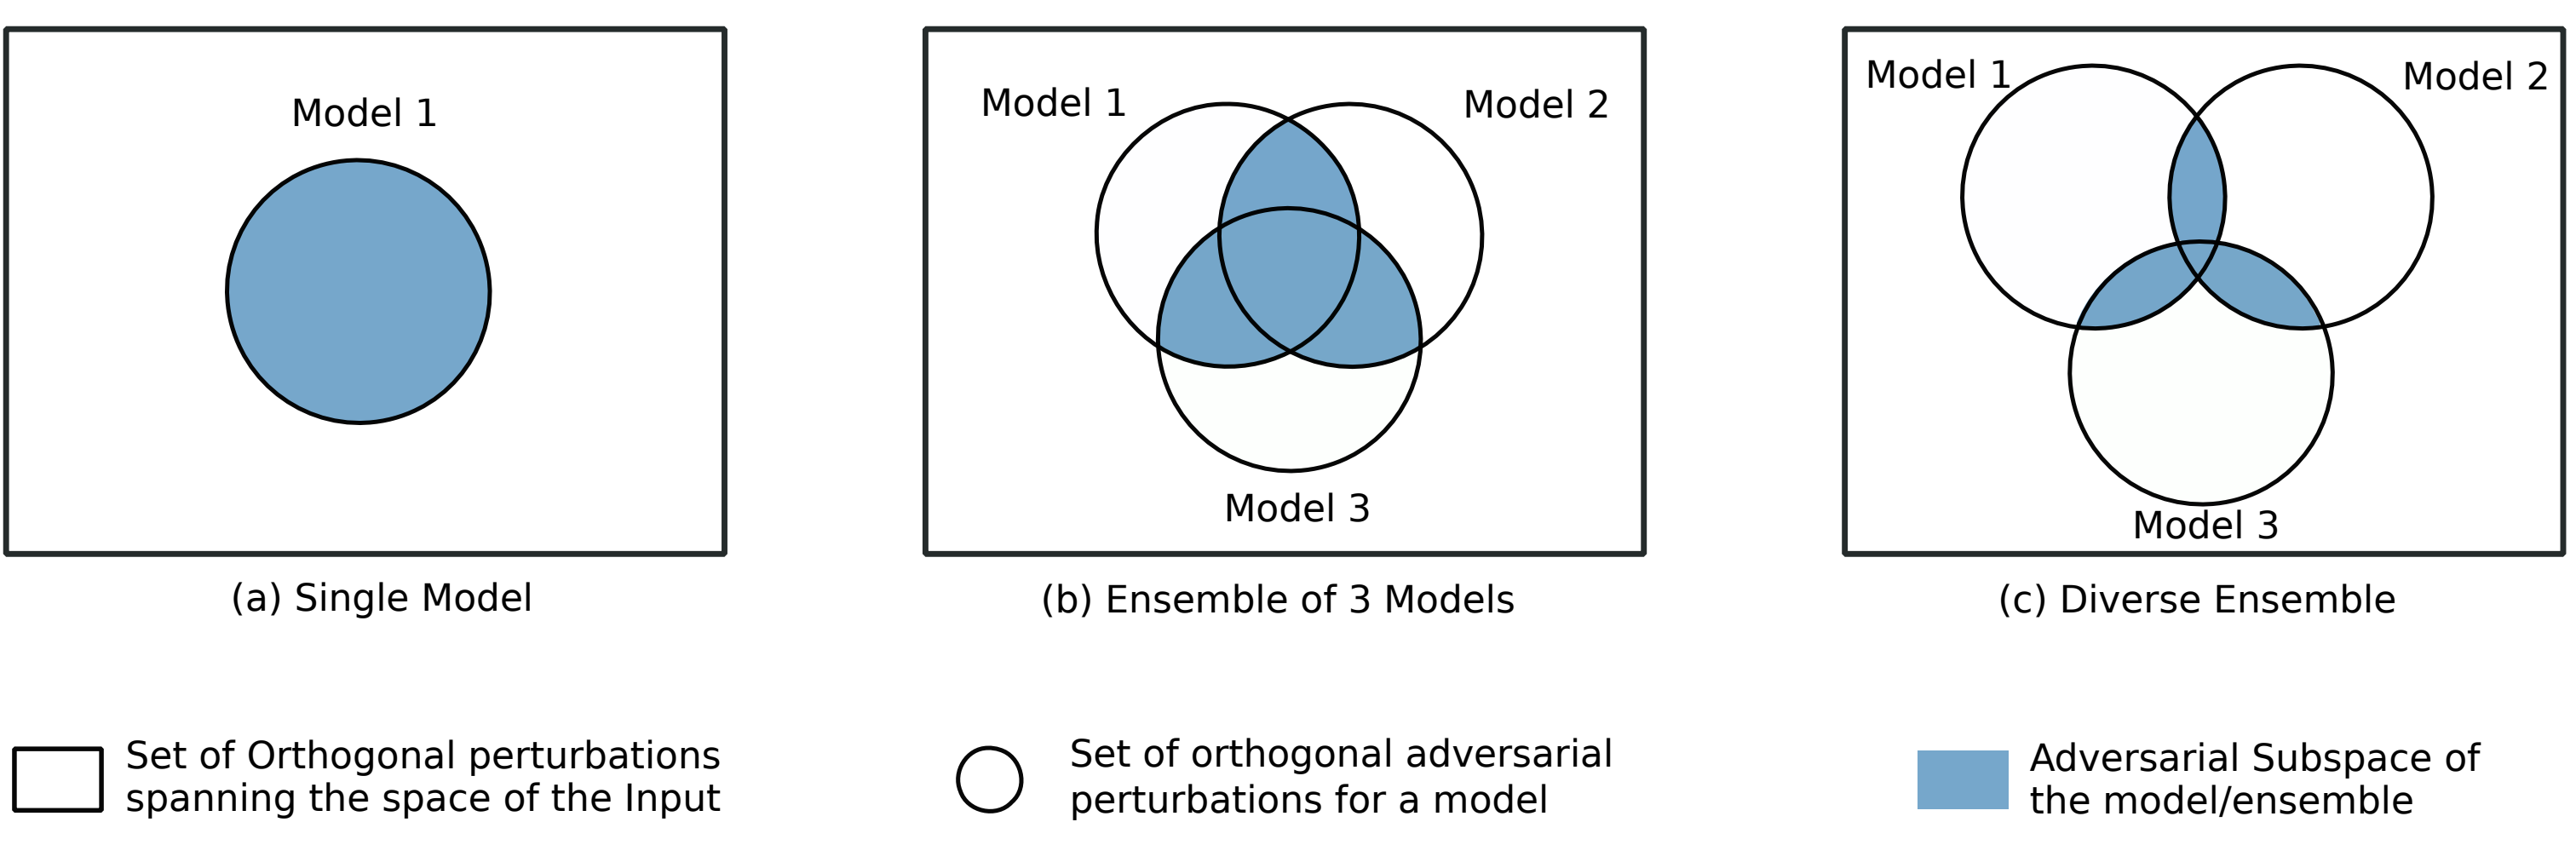
\includegraphics[width=\linewidth]{01-images/06-ending/venn_diversity_training.png}
    \caption{``Venn diagram illustrations of the adversarial subspace of (a) single model (b) Ensemble of 3 models and (c) Diverse Ensemble. Our goal is to reduce the overlap in the adversarial subspaces of the models in the ensemble as shown in (c)'' \cite{kariyappa_improving_2019}}
    \label{fig:venn diversity training}
\end{figure}

\subsubsection{Detektion von Adversarial Attacks}
Paula Harder und ihr Team haben in ihrer Arbeit SpectralDefense: Detecting Adversarial Attacks on CNNs in the Fourier Domain, \cite{harder_spectraldefense_2021} eine  Methode zur Detektion von Adversarial Attacks vorgestellt. Die Detektion solcher Attacken dient als Verteidigungsstrategie, um potenziellen Attacke zu verhindern. In ihrer Untersuchung werden die Fourier-Transformation von Bild- und Feature-Map-Daten genutzt, um zwischen normalen und manipulierten Bildern zu unterscheiden. Dabei werden zwei Ansätze verfolgt: Der erste Ansatz fokussiert sich auf die Analyse des Magnituden-Spektrums der Eingangsbilder, während der zweite Ansatz zusätzlich die Phase der Fourier-Koeffizienten in verschiedenen Netzwerkschichten berücksichtigt.

\subsubsection{Bildmaske}
In den beiden verwendeten Datensätzen Hirntumor und COVIDx sind für die Klassifikation unwichtige schwarze Pixel im Hintergrund vorhanden, die potenziell eine Angriffsfläche für Adversarial Attacks darstellen. Die ausserhalb des Interessensbereichs liegenden schwarzen Pixel enthalten keine für die Klassifikationsaufgabe relevanten Informationen. Um dieses Problem zu adressieren, schlagen wir die Verwendung einer Bildmaske vor. Die Verwendung einer solchen Maske würde dem Modell die Möglichkeit bieten, sich ausschliesslich auf die wesentlichen Bereiche des Bildes zu konzentrieren, in denen relevante Informationen für die Klassifikation vorhanden sind. Die Verwendung einer solchen Maske könnte dazu führen, dass das Modell Perturbationen ausblendet und somit die Angriffsfläche der Perturbationen verringert.

\subsection{Ein Wort zu Technology Credulity}
Sommer \cite{sommer_gesellschaftliche_2024} erklärt in seinem Modul über die gesellschaftlichen Auswirkungen von KI Design, dass im Optimalfall ein Mensch immer direkt in den Entscheidungsprozess eingebunden ist und dass dieser Mensch nicht auf die bisherige Leichtgläubigkeit der Technik hereinfällt. In der Praxis neigt der Mensch jedoch dazu, Ermüdungserscheinungen zu zeigen, wenn er ständig mit ähnlichen Entscheidungen konfrontiert wird. Darüber hinaus ist der Mensch als direkte Folge des gewinnorientierten Denkens teuer und wird nur minimal in solche Systeme eingebunden, was zu weitgehend autonomen Systemen führt.

Daher ist es von entscheidender Bedeutung darauf hinzuweisen, dass Experten, die ähnliche Krankheitserkennungssysteme verwenden, sich auch in Zukunft der Tatsache bewusst sein werden, dass solche Systeme auch bei Vorhandensein oder Nichtvorhandensein von \acrlong{uap} nicht vollständig exakt sind und dass sie als Experten dieser Leichtgläubigkeit zum Opfer fallen könnten. Diese Experten sollten unbedingt \gls{human-in-the-loop} bleiben und den Output dieser Modelle sowie die eigene Nutzung dieser Systeme stets kritisch hinterfragen.